\section*{CHAPTER 3: SYSTEM ANALYSIS AND DESIGN}
\addcontentsline{toc}{section}{\numberline{}CHAPTER 3: SYSTEM ANALYSIS AND DESIGN}
\setcounter{section}{3}
\setcounter{subsection}{0}
\setcounter{figure}{0}
\setcounter{table}{0}

This chapter translates the conceptual goals of the FootField platform into concrete engineering specifications. It details the functional requirements, identifies system actors, presents use case scenarios, and outlines the architectural and database designs.

\subsection{Requirements Analysis}
\subsubsection{Functional Requirements}
The platform is designed to serve three distinct primary actors, each with specific privileges and functional needs:

\textbf{1. Provider Admin (Super Admin):}
\begin{itemize}
    \item \textbf{Tenant Management:} Ability to create, suspend, or delete tenant (facility owner) accounts.
    \item \textbf{Package Management:} Ability to define subscription plans (e.g., Basic, Premium) that limit the number of fields or staff accounts a tenant can create.
    \item \textbf{Global Dashboard:} View aggregated revenue metrics and system-wide usage statistics.
\end{itemize}

\textbf{2. Tenant Admin (Facility Owner \& Staff):}
\begin{itemize}
    \item \textbf{Field Management:} Create and manage football fields, defining their type (5-a-side, 7-a-side) and hourly pricing strategies.
    \item \textbf{Schedule Viewer:} Access an interactive time-grid schedule to visually monitor all bookings across different fields on any given day.
    \item \textbf{QR Check-in:} Use the native mobile application to scan customer QR tickets and automatically update the booking status to "Completed".
    \item \textbf{Financial Reporting:} Generate daily and monthly revenue reports and print invoices.
\end{itemize}

\textbf{3. Customer (End-User):}
\begin{itemize}
    \item \textbf{Availability Search:} Browse available time slots for specific football fields.
    \item \textbf{AI Interaction:} Chat with the Gemini AI virtual assistant to request field recommendations or make bookings using natural language.
    \item \textbf{Online Payment:} Securely pay for bookings via VNPay.
    \item \textbf{Ticket Retrieval:} Receive and display an electronic QR code ticket upon successful booking.
\end{itemize}

\subsubsection{Non-Functional Requirements}
\begin{itemize}
    \item \textbf{Data Security:} Strict isolation of tenant data using the \texttt{tenant\_id} foreign key in all relevant database queries.
    \item \textbf{Performance:} API response times must remain under 500ms for standard database queries to ensure a seamless booking experience.
    \item \textbf{Availability:} The system must maintain 99.9\% uptime, facilitated by cloud-native deployment on Render and Aiven.
\end{itemize}

\subsection{Use Case Scenarios}

To visualize the interactions between the actors and the system, a comprehensive Use Case Diagram is established.

% [PLACEHOLDER FOR USE CASE DIAGRAM]
% \begin{figure}[H]
%     \centering
%     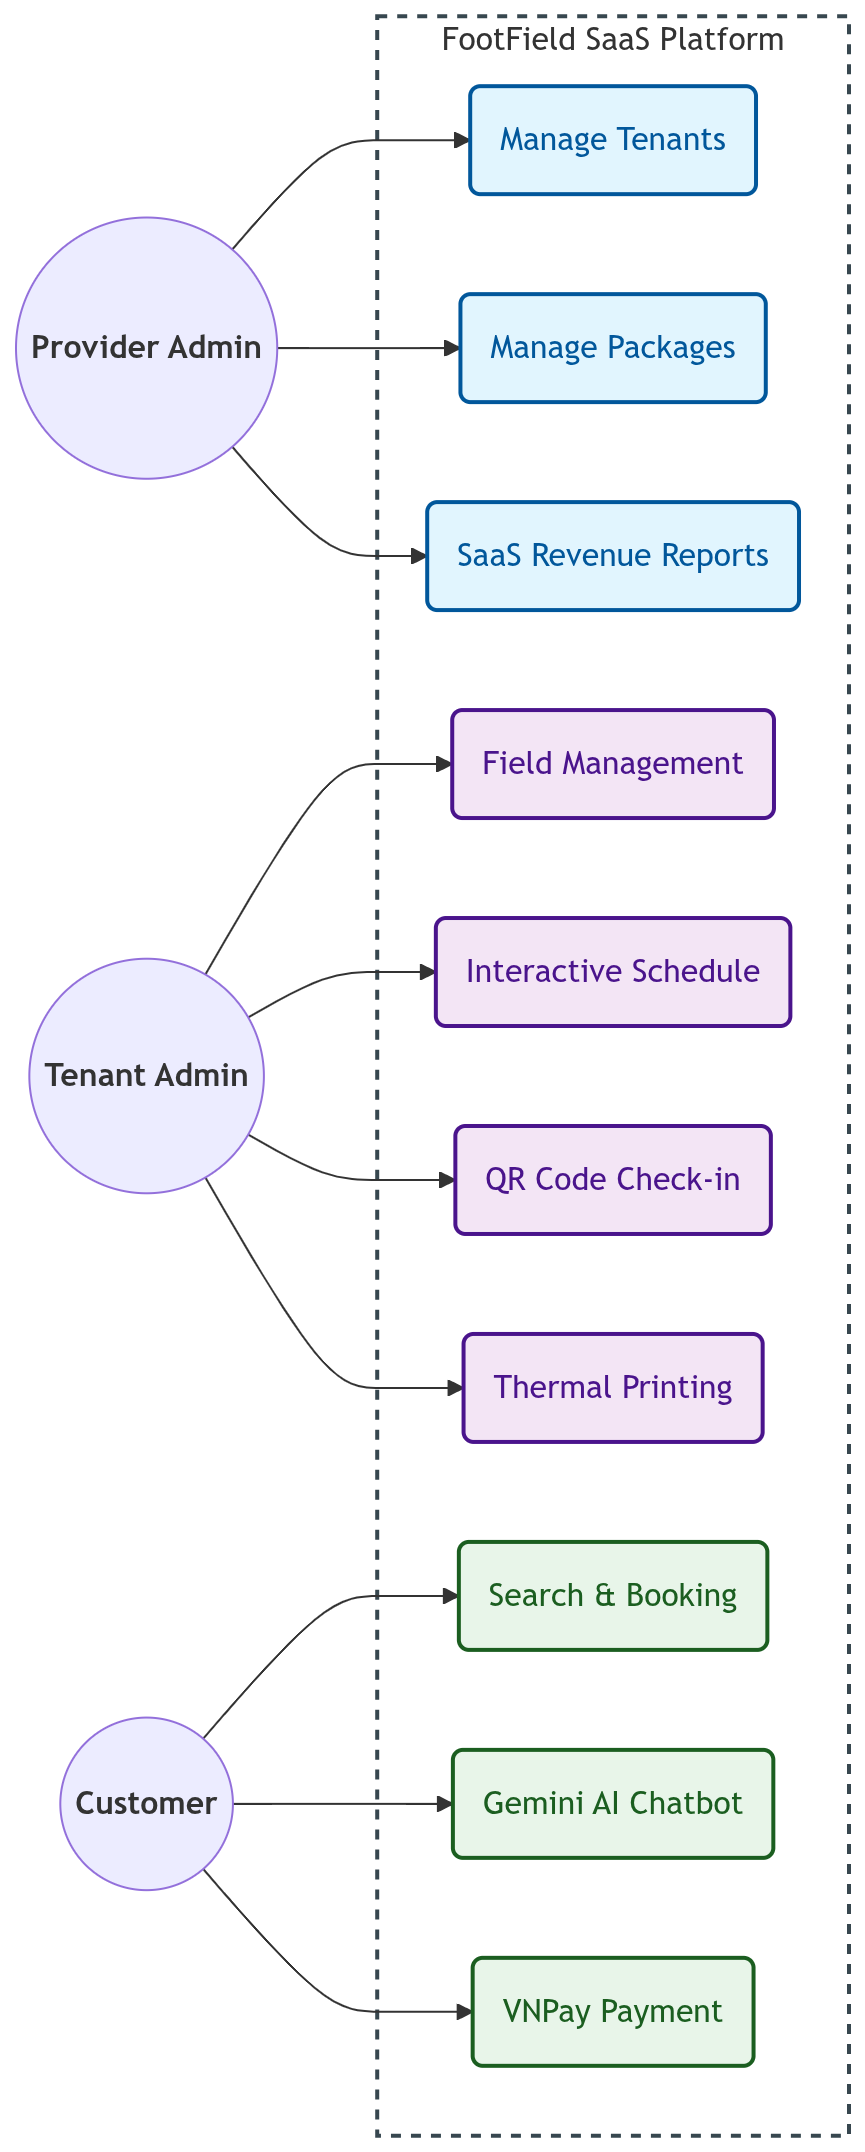
\includegraphics[width=0.9\textwidth]{Figures/usecase_diagram.png}
%     \caption{General Use Case Diagram for FootField System}
%     \label{fig:usecase}
% \end{figure}

\subsubsection{Detailed Use Case: AI-Assisted Booking}
\begin{itemize}
    \item \textbf{Actor:} Customer
    \item \textbf{Precondition:} The customer is on the Tenant's specific storefront URL.
    \item \textbf{Main Flow:}
    \begin{enumerate}
        \item Customer opens the AI Chatbot interface and inputs: "I need a 7-a-side field tomorrow at 18:00".
        \item The system sends the prompt to the Google Gemini API.
        \item The AI recognizes the intent and triggers the \texttt{check\_availability} function.
        \item The system queries the database and returns available fields to the AI.
        \item The AI informs the customer of the available options and asks for confirmation to book.
        \item Customer confirms. The AI triggers the \texttt{create\_booking} function.
        \item The system generates a booking record with "Pending" status and returns a payment link.
    \end{enumerate}
\end{itemize}

\subsubsection{Detailed Use Case: QR Code Check-in}
\begin{itemize}
    \item \textbf{Actor:} Tenant Staff
    \item \textbf{Precondition:} Staff is logged into the Capacitor Android app; Customer has a valid QR ticket.
    \item \textbf{Main Flow:}
    \begin{enumerate}
        \item Staff taps the "Scan QR" button on the mobile app.
        \item The Capacitor camera plugin opens the native device camera.
        \item Staff scans the customer's QR code.
        \item The app decodes the booking ID and sends an API request to the backend.
        \item The system verifies the booking status. If valid, it updates the status to "Completed".
        \item The app displays a success message to the staff.
    \end{enumerate}
\end{itemize}

\subsection{Database Design and ERD}

The database is built on a robust relational model to ensure data integrity. The core of the multi-tenant architecture is the enforcement of the \texttt{tenant\_id} relationship.

% [PLACEHOLDER FOR ERD DIAGRAM]
% \begin{figure}[H]
%     \centering
%     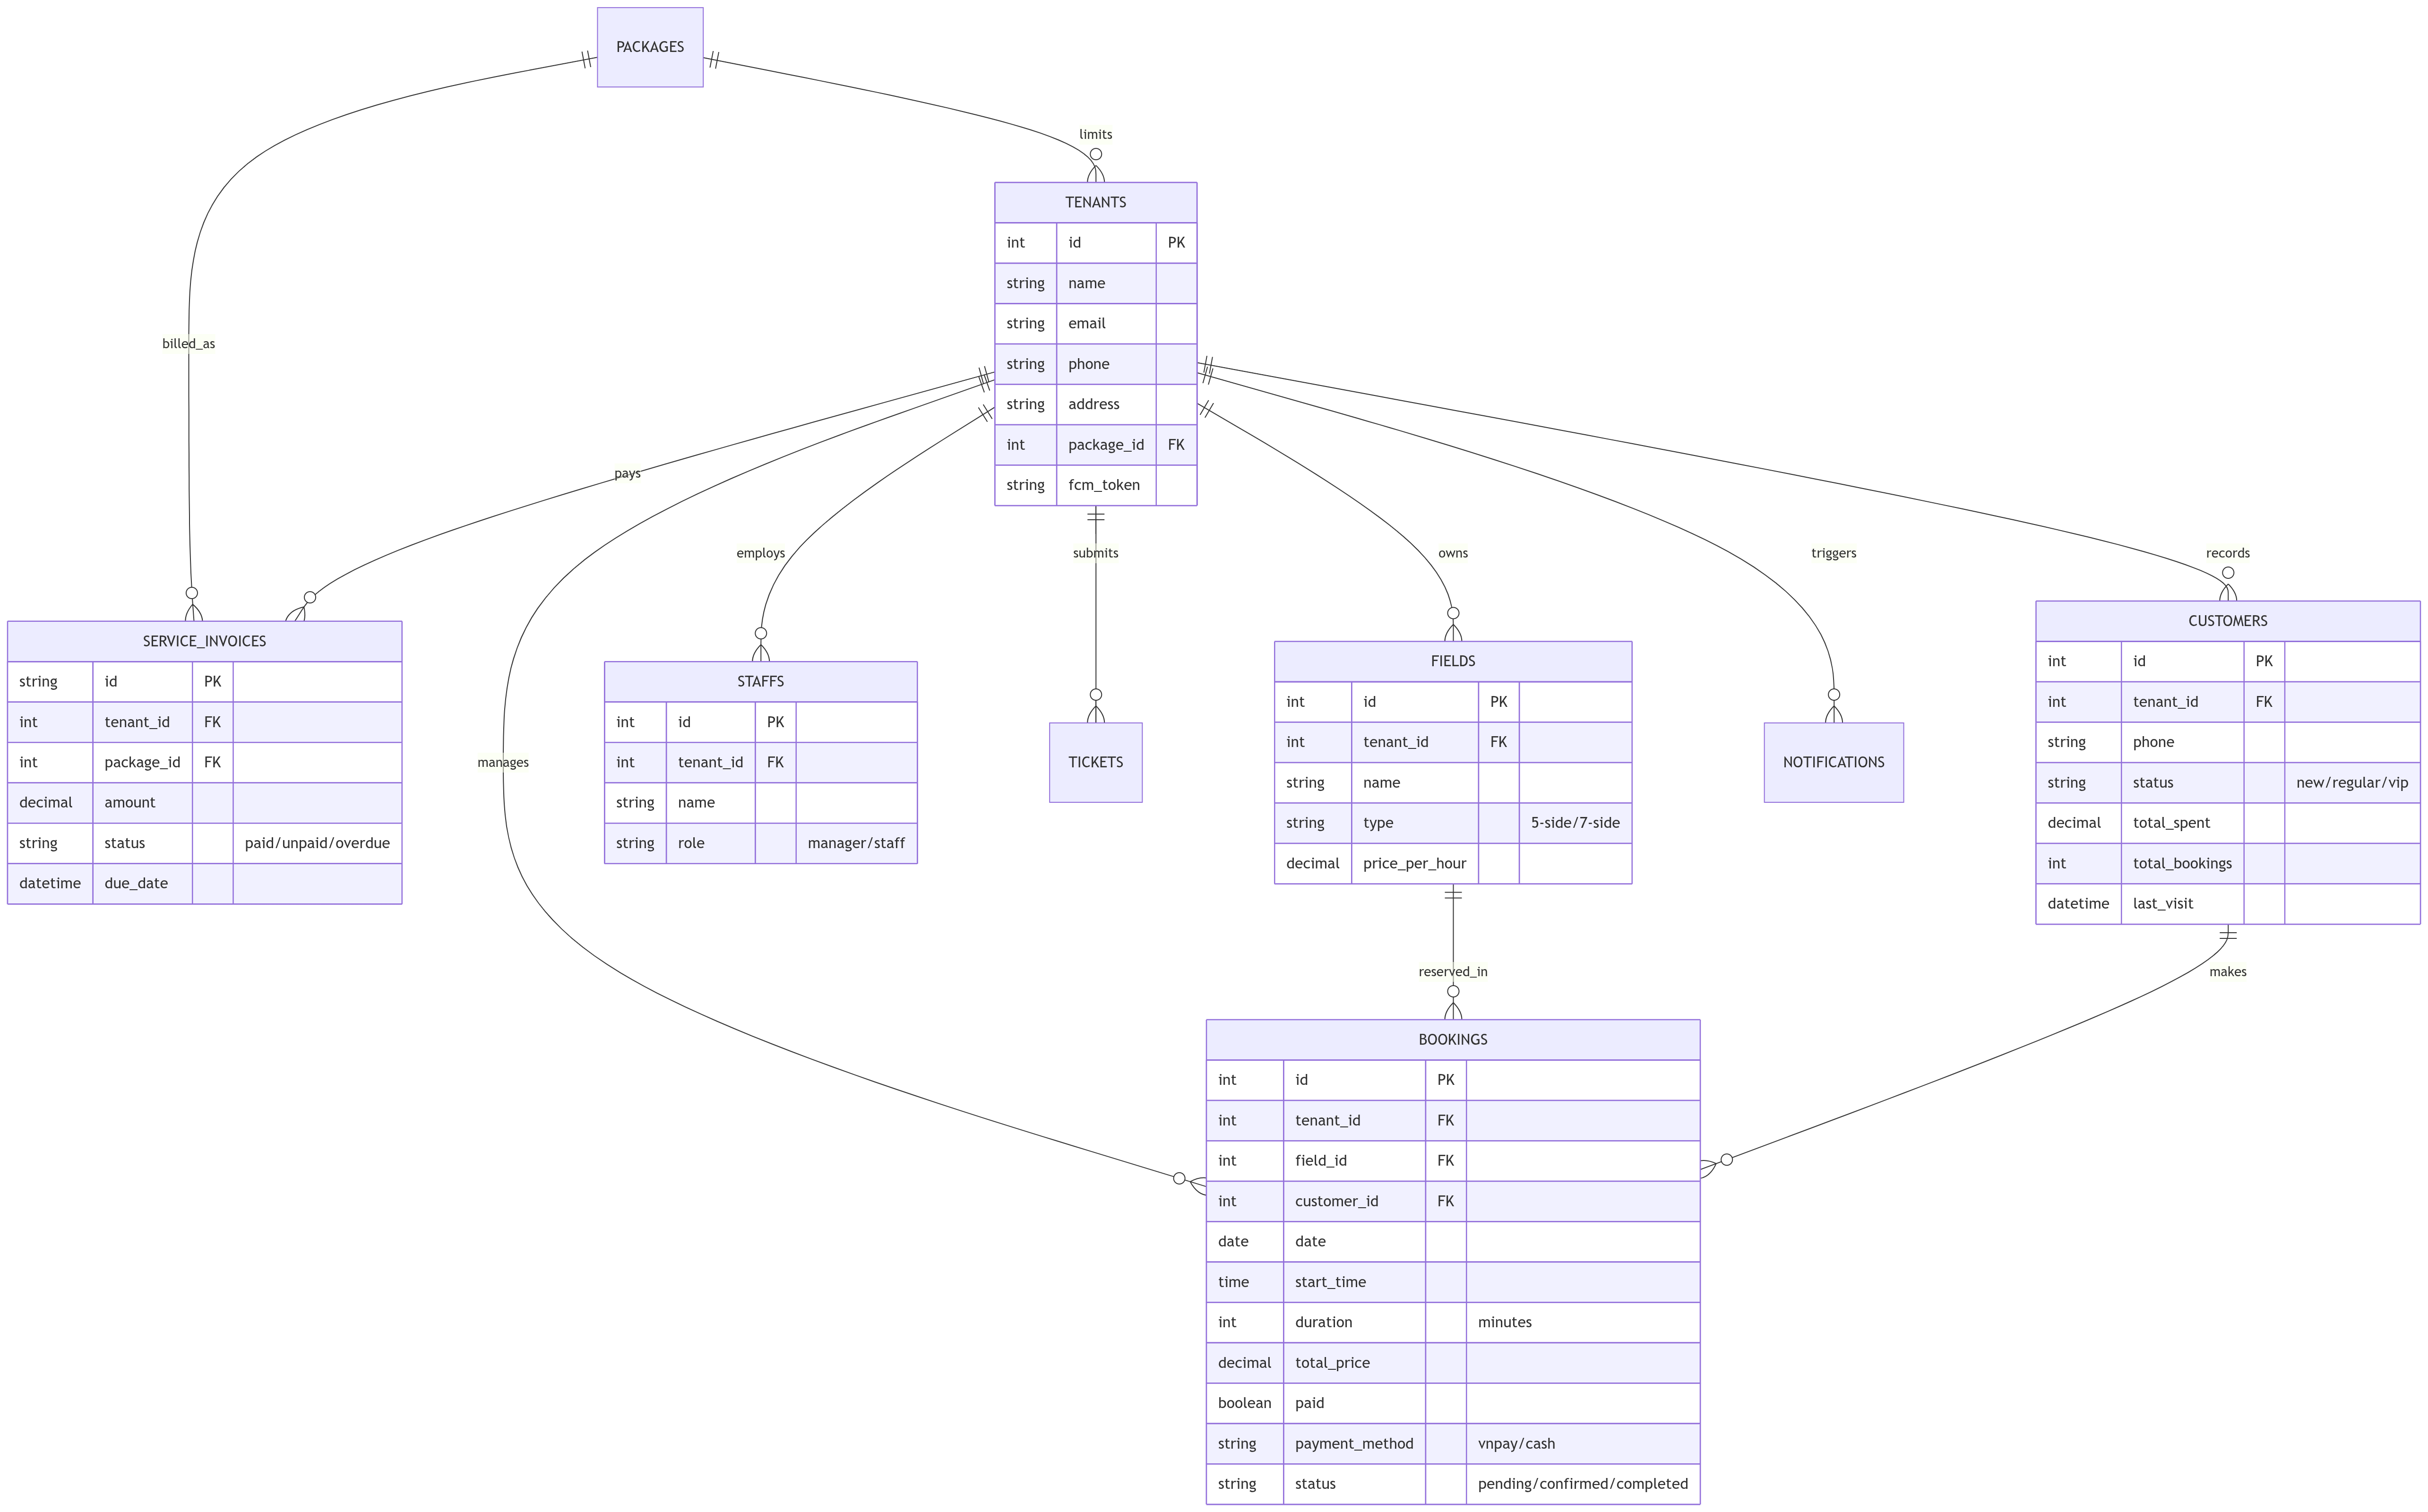
\includegraphics[width=1\textwidth]{Figures/erd_diagram.png}
%     \caption{Entity-Relationship Diagram (ERD)}
%     \label{fig:erd}
% \end{figure}

\subsubsection{Table Schemas}
\textbf{1. Table: tenants}
\begin{itemize}
    \item \texttt{id} (INT, Primary Key): Unique identifier for the facility owner.
    \item \texttt{name} (VARCHAR): Name of the facility.
    \item \texttt{domain} (VARCHAR): Unique subdomain for the customer storefront.
    \item \texttt{package\_id} (INT, Foreign Key): Links to the subscription packages table.
\end{itemize}

\textbf{2. Table: fields}
\begin{itemize}
    \item \texttt{id} (INT, Primary Key)
    \item \texttt{tenant\_id} (INT, Foreign Key): Ensures the field belongs to a specific tenant.
    \item \texttt{name} (VARCHAR): e.g., "Field A".
    \item \texttt{type} (VARCHAR): e.g., "5-a-side".
    \item \texttt{price\_per\_hour} (DECIMAL): Standard hourly rate.
\end{itemize}

\textbf{3. Table: bookings}
\begin{itemize}
    \item \texttt{id} (INT, Primary Key)
    \item \texttt{tenant\_id} (INT, Foreign Key)
    \item \texttt{field\_id} (INT, Foreign Key)
    \item \texttt{customer\_name} (VARCHAR), \texttt{customer\_phone} (VARCHAR)
    \item \texttt{start\_time} (DATETIME), \texttt{end\_time} (DATETIME)
    \item \texttt{status} (ENUM): 'pending', 'confirmed', 'completed', 'cancelled'.
\end{itemize}

\subsection{System Sequence Diagrams}

Sequence diagrams illustrate the dynamic interaction between system components over time. Two critical workflows are defined below.

% [PLACEHOLDER FOR AI SEQUENCE DIAGRAM]
% \begin{figure}[H]
%     \centering
%     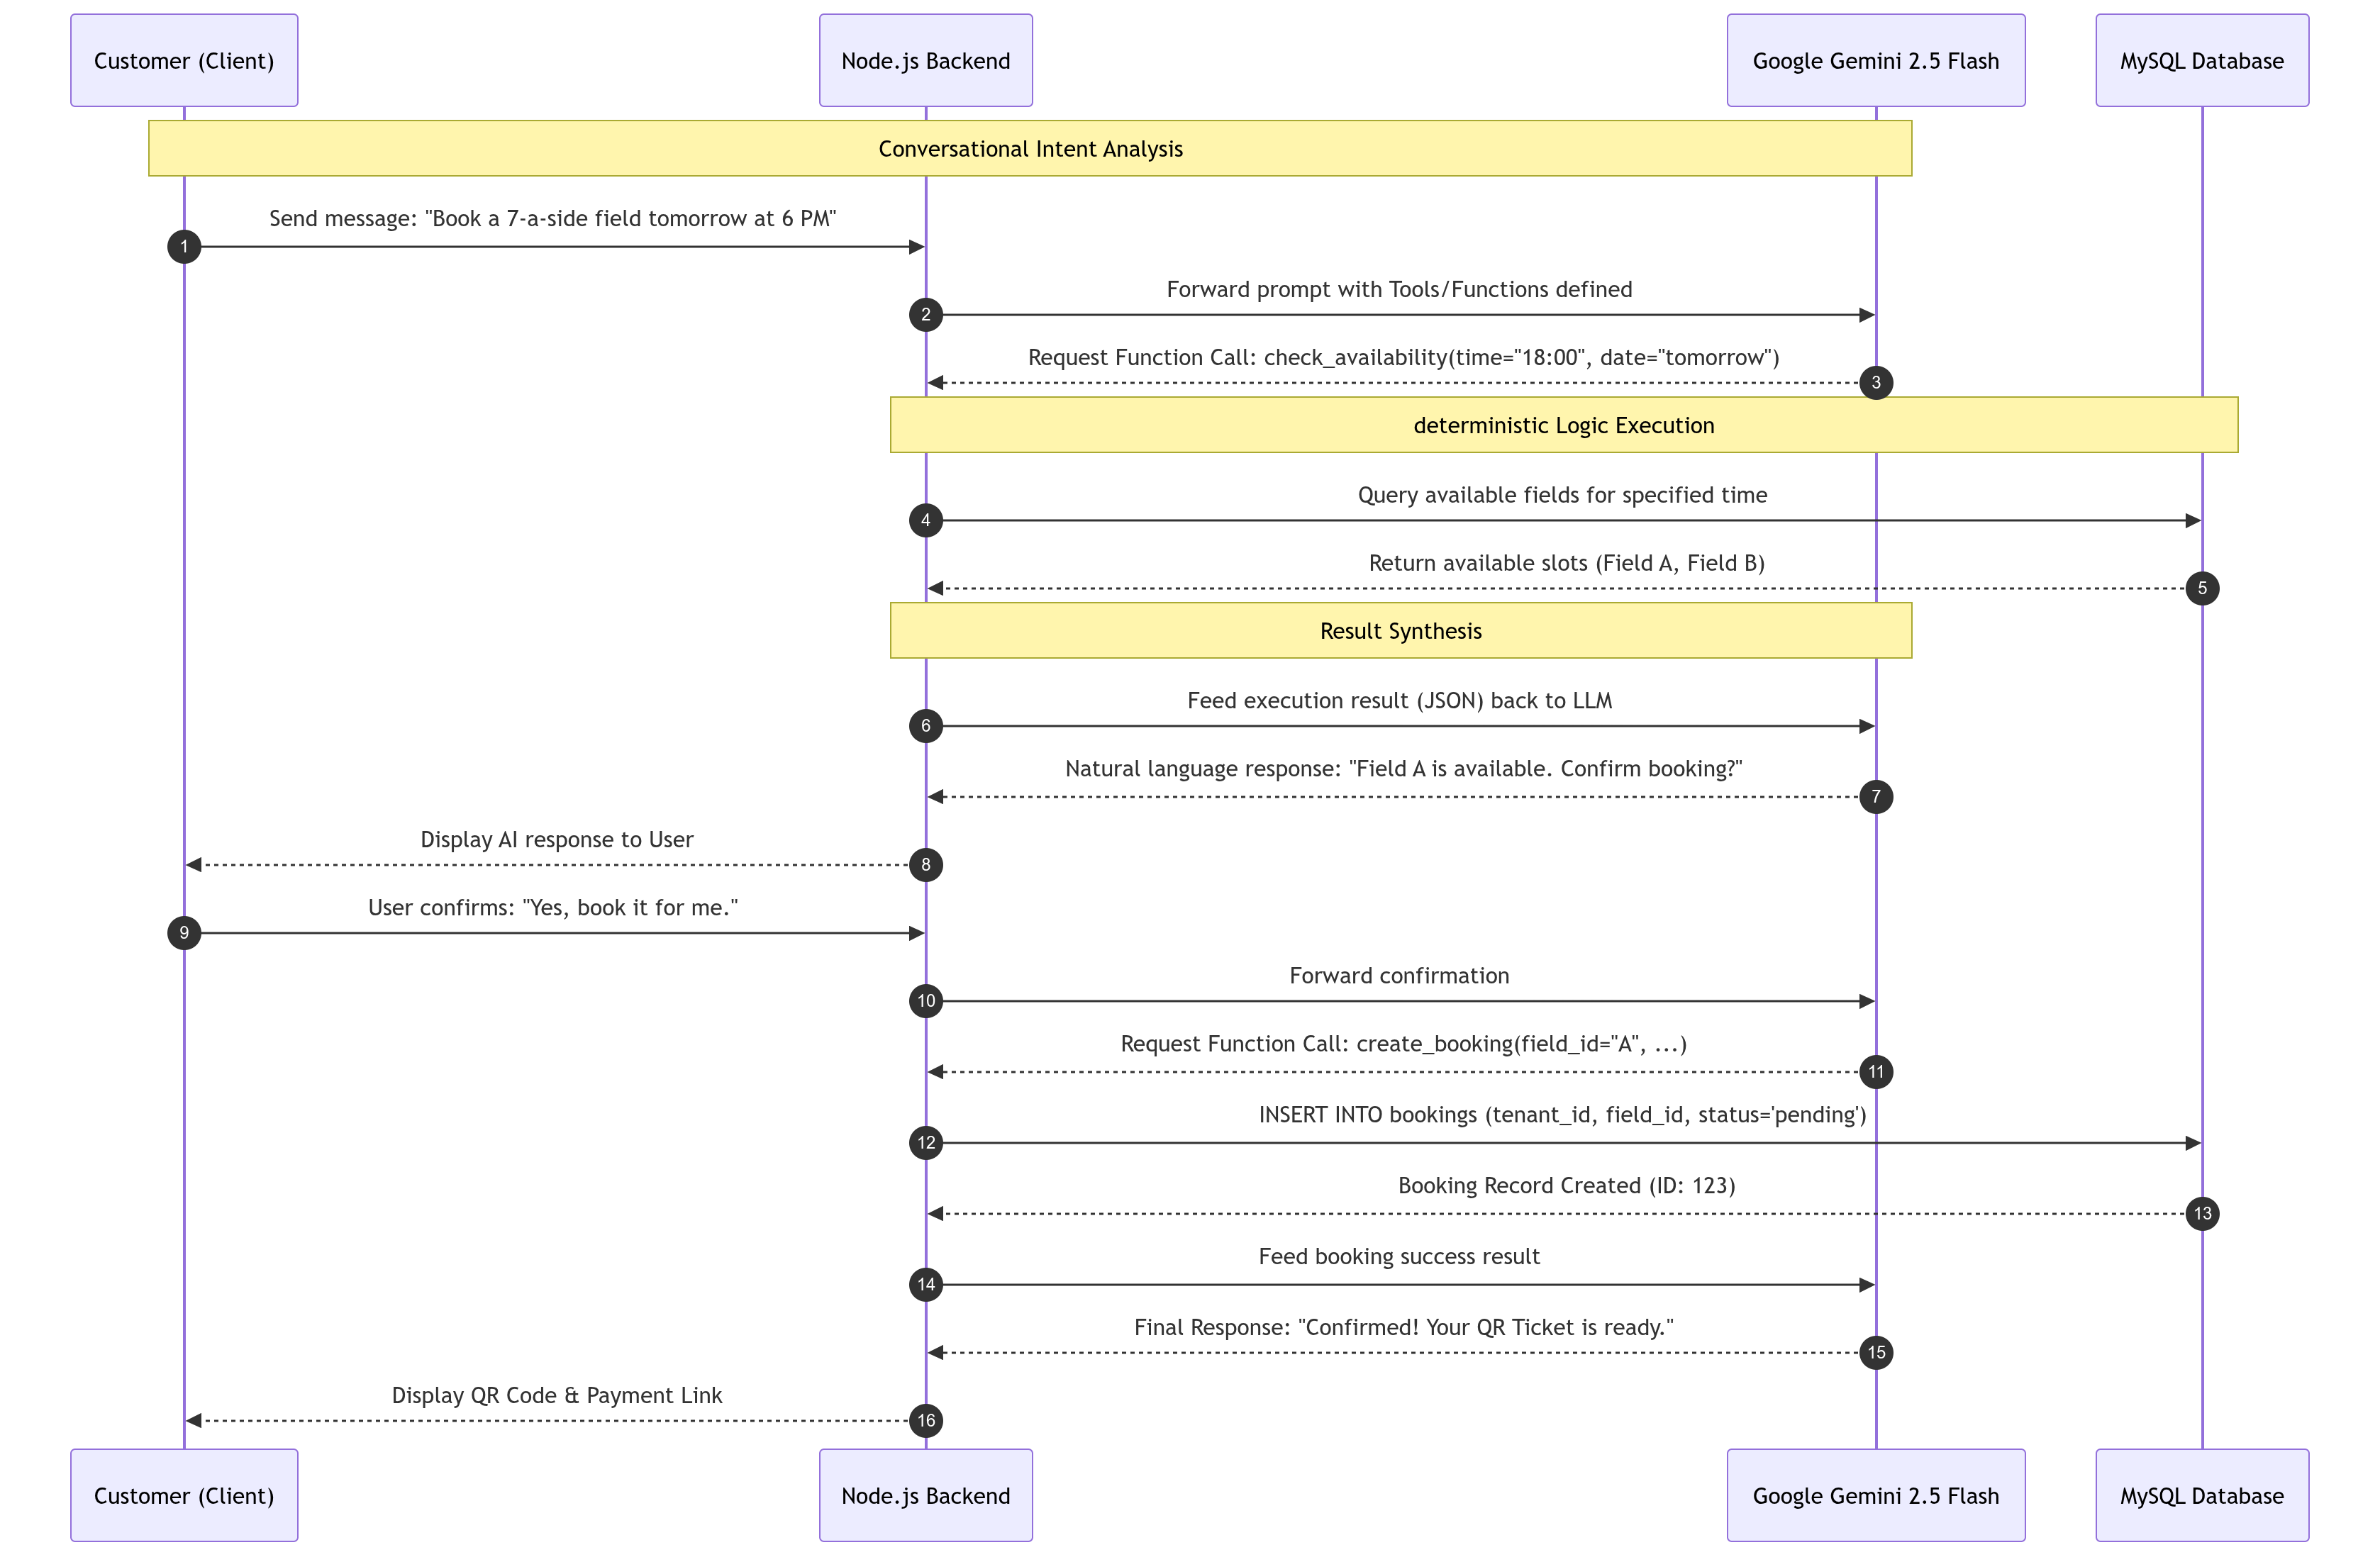
\includegraphics[width=0.9\textwidth]{Figures/seq_ai_booking.png}
%     \caption{Sequence Diagram: AI-Assisted Booking Workflow}
%     \label{fig:seq_ai}
% \end{figure}

The \textbf{AI Booking Sequence} involves the Customer (Client), the Node.js Server, the MySQL Database, and the Google Gemini API. The server acts as an intermediary, utilizing Function Calling to execute database reads/writes on behalf of the AI before returning the final natural language response to the client.

% [PLACEHOLDER FOR VNPAY SEQUENCE DIAGRAM]
% \begin{figure}[H]
%     \centering
%     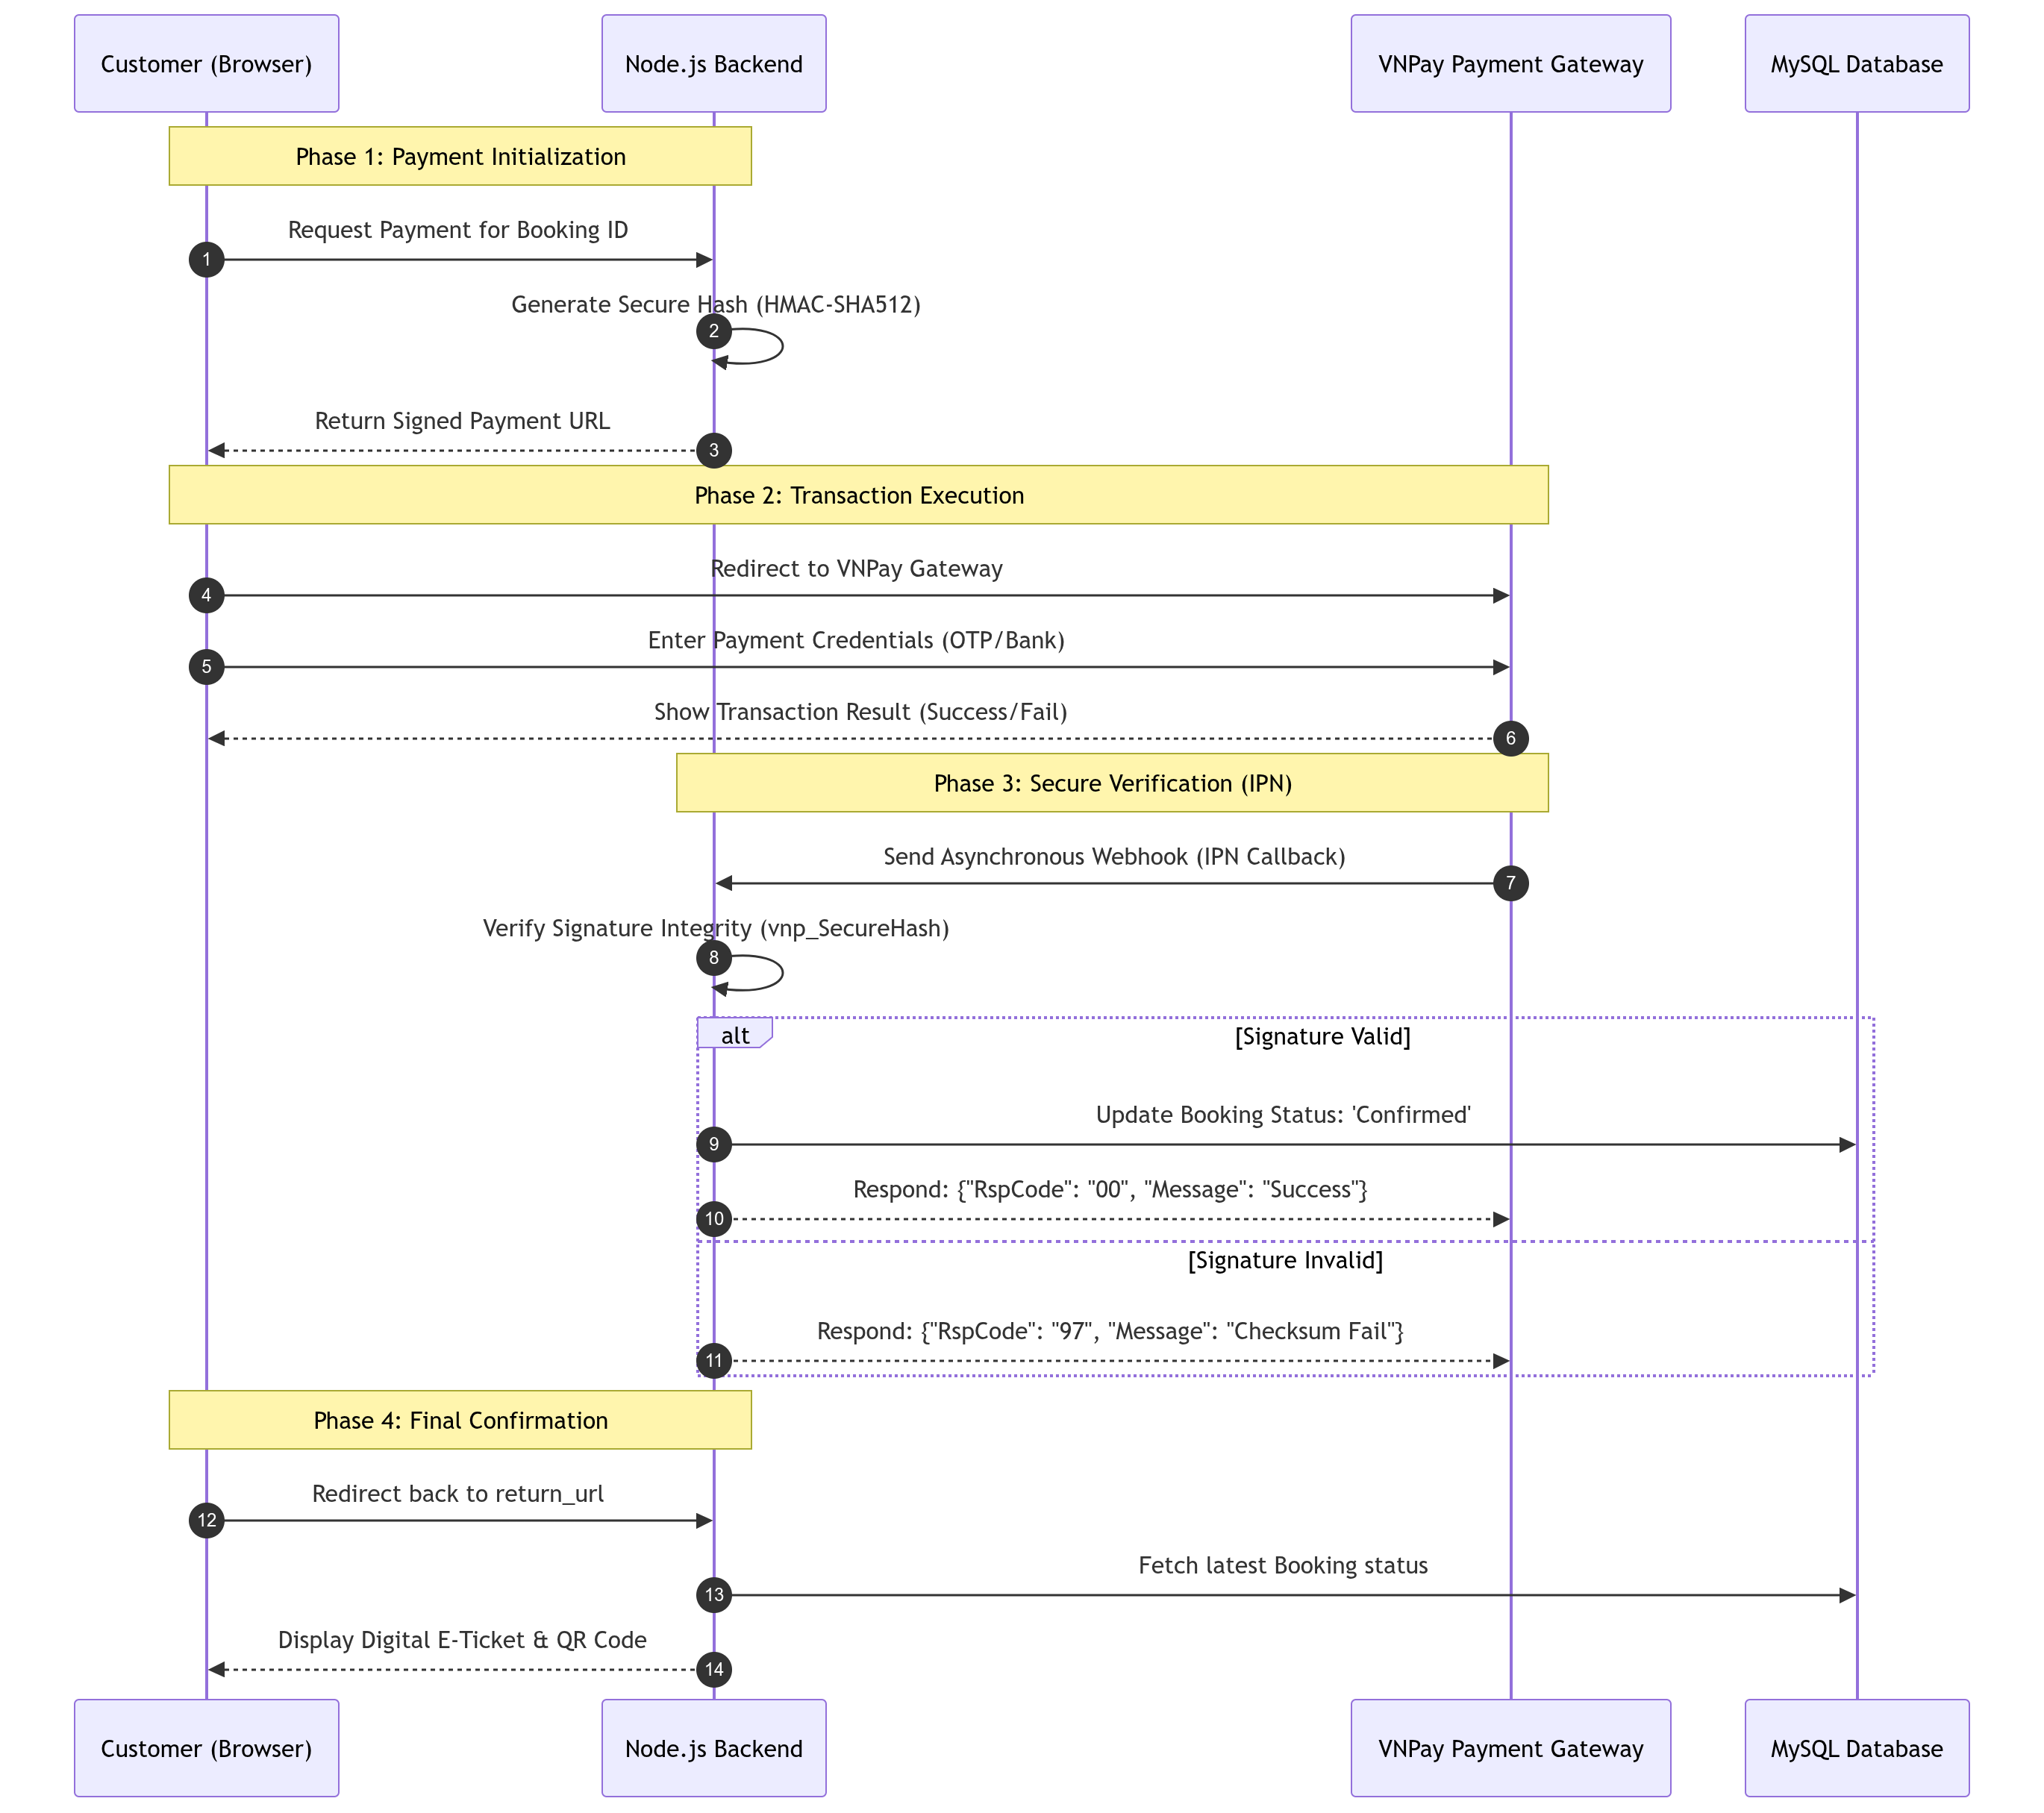
\includegraphics[width=0.9\textwidth]{Figures/seq_vnpay.png}
%     \caption{Sequence Diagram: VNPay Payment Integration}
%     \label{fig:seq_vnpay}
% \end{figure}

The \textbf{VNPay Sequence} demonstrates the secure payment handshake. Upon booking creation, the server generates a signed VNPay URL. The client is redirected to VNPay to enter payment details. Crucially, VNPay sends an asynchronous IPN (Instant Payment Notification) callback to the Node.js server to verify the transaction independently of the client-side redirect, ensuring that the booking status is updated securely.